\documentclass[12pt,a4paper]{report}
\usepackage[utf8]{inputenc}
\usepackage{amsmath}
\usepackage{amssymb}
\usepackage{graphicx}
\usepackage{geometry}
\usepackage[hidelinks]{hyperref}  % For clickable references
\usepackage[capitalise]{cleveref}  % For intelligent cross-referencing
\usepackage[english]{babel}

\usepackage{makecell}
\usepackage{caption}
\usepackage{array}
\usepackage{listings}
\usepackage{titlesec}

\graphicspath{{C:/Users/frabb/OneDrive - Cal Poly/Documents (Cloud)/0 CALPOLY/000Thesis/Chapters/Images/}}

\geometry{
  top=1in,
  bottom=1in,
  left=1.5in,
  right=1in
}

% Remove space before equations only
\makeatletter
\g@addto@macro\normalsize{%
	\setlength\abovedisplayskip{-10pt}
	\setlength\abovedisplayshortskip{-10pt}
}
\makeatother

% Updated list settings
\usepackage{enumitem}
\setlist[itemize]{nosep, leftmargin=*}
\setlist[enumerate]{nosep, leftmargin=*}

% Remove space before lists
\usepackage{etoolbox}
\BeforeBeginEnvironment{itemize}{\vspace{-\baselineskip}}
\BeforeBeginEnvironment{enumerate}{\vspace{-\baselineskip}}

\setlength{\parskip}{\baselineskip}
\titlespacing*{\section}{0pt}{0pt}{0pt}
\titlespacing*{\section}{0pt}{0pt}{-10pt}
\titlespacing*{\subsection}{0pt}{0pt}{-10pt}

\captionsetup[table]{skip=0pt}

\usepackage{xcolor}

\definecolor{codegreen}{rgb}{0,0.6,0}
\definecolor{codegray}{rgb}{0.5,0.5,0.5}
\definecolor{codepurple}{rgb}{0.58,0,0.82}
\definecolor{backcolour}{rgb}{0.95,0.95,0.92}

\lstdefinestyle{mystyle}{
	backgroundcolor=\color{backcolour},   
	commentstyle=\color{codegreen},
	keywordstyle=\color{magenta},
	numberstyle=\tiny\color{codegray},
	stringstyle=\color{codepurple},
	basicstyle=\ttfamily\footnotesize,
	breakatwhitespace=false,         
	breaklines=true,                 
	captionpos=b,                    
	keepspaces=true,                 
	numbers=left,                    
	numbersep=5pt,                  
	showspaces=false,                
	showstringspaces=false,
	showtabs=false,                  
	tabsize=2
}

\lstset{style=mystyle}

\title{Tutorial}
\author{Jakob Frabosilio}
\date{\today}
\setcounter{chapter}{1}
\begin{document}
	
\chapter{Ground-Truth Positioning System} \label{chap:2c}
Testing the accuracy of the proposed iSBL-SF positioning system algorithm requires knowing where the system truly is - thus, a ground-truth positioning system is needed. This system should give the true position of the iSBL array (with some uncertainty), and should be controllable and positionable to allow testing of different locations. 

This chapter details the design of the Fo-SHIP, the ground-truth positioning system for this thesis. First, the inspiration behind the design and previous works that the Fo-SHIP builds off of are discussed. The mechanical and electrical design are detailed, and the manufacturing and assembly are shown. Then, the software running the Fo-SHIP is documented. Lastly, the calibration, testing, and validation of the system are described.

\section{Design Inspiration and Previous Works} \label{sec:2s1}
The ground-truth positioning system for this thesis is modeled after a unique actuator henceforth known as a “stacked hexapod platform,” as first described in a publication from NASA Langley Research Center \cite{nasaSSPpaper}. In the paper, Balaban, Cooper, and Komendera constructed an actuator they called an “Assembler” made of multiple Stewart platforms that are vertically stacked upon each other. The mechanism is a novel attempt at creating a robotic system that can assemble structures in space, and is the only one of its kind. A picture of their actuator is shown in Figure \ref{fig:nasassp} below.

\begin{figure}[htbp]
	\centering
	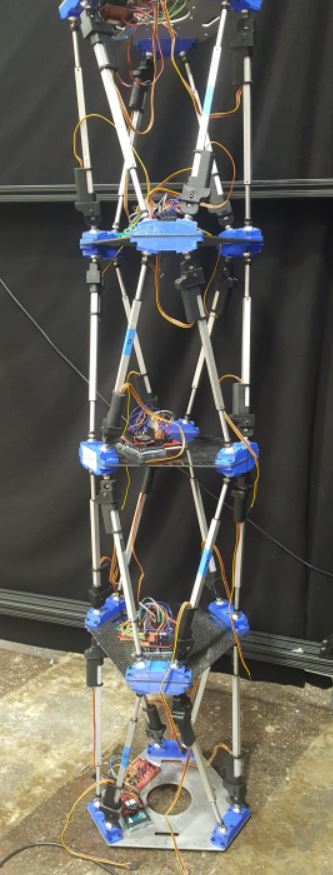
\includegraphics[width=0.5\textwidth]{nasassp}
	\caption{Stacked Stewart platform from Balaban, Cooper, and Komendera \cite{nasaSSPpaper}}
	\label{fig:nasassp}
\end{figure}

\subsection{Stewart Platform Origins} \label{ssec:2s1s1}
A Stewart platform, also known as a hexapod or Stewart-Gough platform, is a six degree-of-freedom (DOF) actuator invented in the mid-20th century. The true inventor of the platform is disputed. In 1954, Eric Gough, an automotive engineer, designed a hexapod platform to test different loading conditions on tires \cite{parallelorigins}. A picture of his platform is shown in Figure \ref{fig:goughplatform} below.

\begin{figure}[htbp]
	\centering
	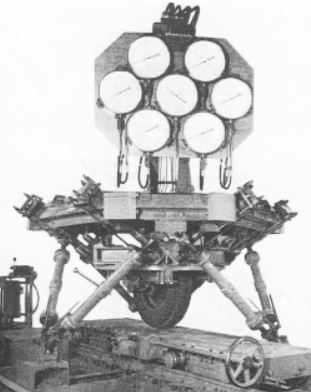
\includegraphics[width=0.5\textwidth]{goughplatform}
	\caption{Gough’s hexapod platform \cite{parallelorigins}}
	\label{fig:goughplatform}
\end{figure}

\vspace{1ex}
Eleven years later, D. Stewart (an engineer whose full first name appears to be unknown) published a paper proposing a platform with six degrees of freedom meant for use in flight simulators. In his paper, he noted correspondence with Gough \cite{stewartpaper}. An image of his proposed platform is shown in Figure \ref{fig:stewartOG} below.

\begin{figure}[htbp]
	\centering
	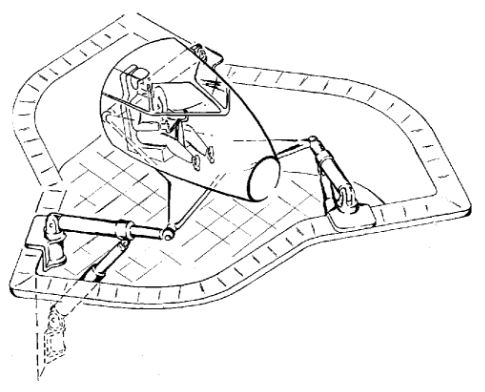
\includegraphics[width=0.5\textwidth]{stewartOG}
	\caption{Stewart’s hexapod platform \cite{stewartpaper}}
	\label{fig:stewartOG}
\end{figure}

Additionally, an engineer named Klaus Cappel independently developed a hexapod platform as a flight simulator for helicopter pilots and constructed a prototype in 1964 \cite{parallelorigins}. An image of Cappel’s platform is shown in Figure \ref{fig:cappelplatform}.

\begin{figure}[htbp]
	\centering
	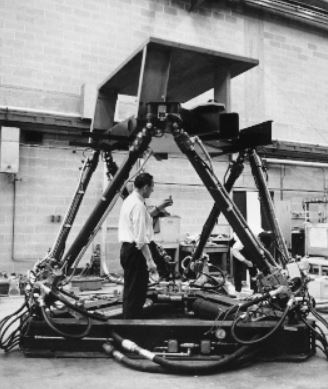
\includegraphics[width=0.5\textwidth]{cappelplatform}
	\caption{Cappel’s hexapod platform \cite{parallelorigins}}
	\label{fig:cappelplatform}
\end{figure}

Despite the independent creations of the platform, Stewart’s name has stuck. Though “Stewart platform” is the most common name of this type of mechanism, the mechanism in this thesis’s implementation will be primarily referred to as a “hexapod."

\subsection{Reinforcement Learning Research} \label{ssec:2s1s2}
As part of an Artificial Intelligence course taken in pursuit of this Master’s degree, a deep reinforcement learning agent was designed to control a stacked hexapod platform \cite{cscpaper}. For this implementation, a custom Gymnasium (a common deep reinforcement learning framework \cite{gymnasium}) environment was developed to represent the kinematics of a stacked hexapod platform. A visualization of the environment is shown in Figure \ref{fig:deepRL} below.

\begin{figure}[htbp]
	\centering
	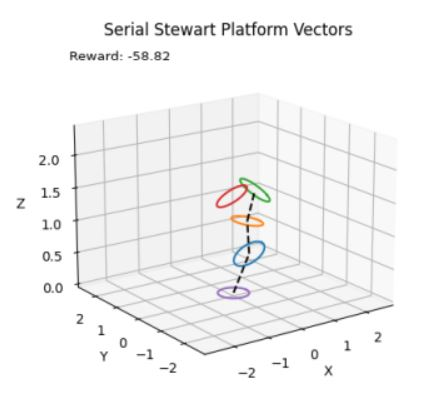
\includegraphics[width=0.5\textwidth]{deepRL}
	\caption{Custom stacked hexapod platform Gymnasium environment \cite{cscpaper}}
	\label{fig:deepRL}
\end{figure}

The location and orientation of a single hexapod platform is dependent on the platform directly beneath it. Two vectors are used per platform: a position vector describes the distance between the centers of the top and bottom of a platform, and an orientation vector describes the vector normal to the surface of the top of the platform. This is a simplified implementation of a hexapod platform; normally, they are described by the six actuators that connect the base and the top. However, the simplified implementation was much easier to work with for a first attempt at deep reinforcement learning. Additionally, the simplified implementation can be related to the true implementation (using six actuators) using kinematics, so the model still moves as a “true” hexapod platform would.

The reinforcement learning attempt ultimately did not succeed due to errors in the Gymnasium implementation (which were identified months after the initial attempt). However, this first attempt at creating a stacked hexapod platform was the inspiration behind the ground-truth positioning system for this thesis. Future plans are to train a deep reinforcement learning agent to control the platform built for this thesis, using an improved Gymnasium environment and interfacing with the real-world system.

\subsection{Inverse Kinematics of a Single Hexapod Platform} \label{ssec:2s1s3}
Much of the inverse kinematics work for this mechanism were derived from previous authors. Notably, a paper by an unknown author from the Wokingham U3A Math Group details an inverse kinematics solution for a hexapod platform controlled by six rotary servos \cite{wokingham}. An art installation named “memememe” improved upon this solution and implemented the design into a single hexapod platform for controlling the motion of a smartphone attached to the end effector \cite{meme}. Lastly, an open-source implementation of a single hexapod platform using an ESP32 was posted online by Nicolas Jeanmonod \cite{nicdoc} \cite{nichub}. This thesis has modified Jeanmonod’s implementation to work with a stacked hexapod platform and some new features and functions were added, but his work is the backbone of the hexapod platform controller. The details of the inverse kinematics of the platform will be described later in Section \ref{ssec:2s5s5}, along with their code implementation.

\subsection{Consideration of Alternative Systems} \label{ssec:2s1s4}
The stacked hexapod platform was one of many contenders for the ground-truth positioning system. The requirements for the ground-truth position system were:

\begin{itemize}[noitemsep,topsep=0pt]
	\item Six degrees of freedom - translation and rotation about XYZ axes
	\item Low cost - this thesis is not funded through grants or external sources
	\item Large range of motion - at least capable of ±0.5m along some translational axis and ±45° about some rotational axis
	\item High accuracy - true position must be within ±1cm of setpoint
\end{itemize}

\noindent The actuators considered were:

\begin{itemize}[noitemsep,topsep=0pt]
	\item Cartesian/gantry robot - a robot constructed from linear actuators (similar to a 3D printer) and a rotating end effector
	\item Articulated arm robot - a robot constructed from rotary actuators (similar to most industrial robotic arms)
	\item Stacked hexapod platform - a robot constructed from stacked hexapod platforms
	\item Cable-driven robot - a robot with a large frame and multiple (6-8) cable-driven actuators that move an end effector in the center of the frame
\end{itemize}

\vspace{2ex}
\noindent The evaluation criteria were:

\begin{itemize}[noitemsep,topsep=0pt,]
	\item Accuracy - is the system capable of high accuracy and repeatability? Higher accuracy is better.
	\item Cost - is the actuator low-cost to design and manufacture? Lower cost is better.
	\item Manufacturability - how feasible is it to make the parts required to the necessary tolerances? Easier manufacturability is better.
	\item Research potential - is it a novel system? More novel and less widely used is better.
	\item Relative size - how large is the system compared to its range of motion? Smaller is better.
	\item Complexity - how many moving parts does the system have?
\end{itemize}

\noindent A Pugh matrix below shows the consideration process. Ultimately, the stacked hexapod platform was chosen due to its low cost, high research potential, and manufacturability. 

\begin{table}[htbp]
	\centering
	\caption{Pugh matrix for ground-truth positioning system actuator}
	\label{tab:pughmatrix}
	\begin{tabular}{|c|c|c|c|c|c|}
		\hline
		\makecell{Criteria} & \makecell{Weight} & \makecell{Cartesian\\robot} & \makecell{Articulated\\robot} & \makecell{Stacked\\hexapod\\platform} & \makecell{Cable-\\-driven\\robot} \\
		\hline
		Accuracy & 3 & Datum & - & - & - \\
		\hline
		Cost & 5 & Datum & + & + & + \\
		\hline
		Manufacturability & 2 & Datum & S & + & - \\
		\hline
		Research potential & 4 & Datum & S & + & + \\
		\hline
		Relative size & 3 & Datum & + & + & S \\
		\hline
		Complexity & 1 & Datum & + & - & - \\
		\hline
		\multicolumn{2}{|c|}{Weighted Sums} & 0 & 6 & 10 & 3 \\
		\hline
	\end{tabular}
\end{table}

The chosen system has been named the “Four-Stacked Hexapod Isometric Platform,” abbreviated as Fo-SHIP. The system is four equally-sized (isometric) hexapod platforms stacked upon each other. As an added bonus, the pronunciation of Fo-SHIP sounds like “faux ship,” which is exactly what this positioner is: a fake version of the submarine that the iSBL-SF system will be eventually deployed on.

\section{Mechanical Design} \label{sec:2s2}
The mechanical design of the Fo-SHIP is inspired by Jeanmonod’s implementation \cite{nicdoc}. His design, shown below, uses six rotary servos sandwiched between two hexagonal plates as the base, and a single hexagonal plate as the top / end effector. Ball joints are used to connect threaded rods to the servo horns and the end effector. The top hexagonal plate is 3D printed and uses heat-set threaded inserts to secure the ball screws, while the base plates appear to be made from composite board material. His design is fully documented and a parts list is available on the project’s GitHub page \cite{nichub} A CAD rendering and physical model of Jeanmonod's implementation can be seen in Figures \ref{fig:nicplatform} and \ref{fig:nicplatform2}. 

\begin{figure}[htbp]
	\centering
	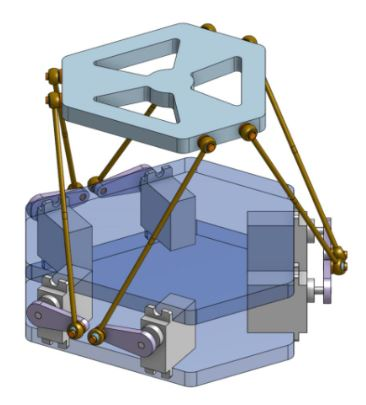
\includegraphics[width=0.5\textwidth]{nicplatform}
	\caption{Jeanmonod’s implementation of a single hexapod platform, CAD model \cite{nichub}}
	\label{fig:nicplatform}
\end{figure}

\begin{figure}[htbp]
	\centering
	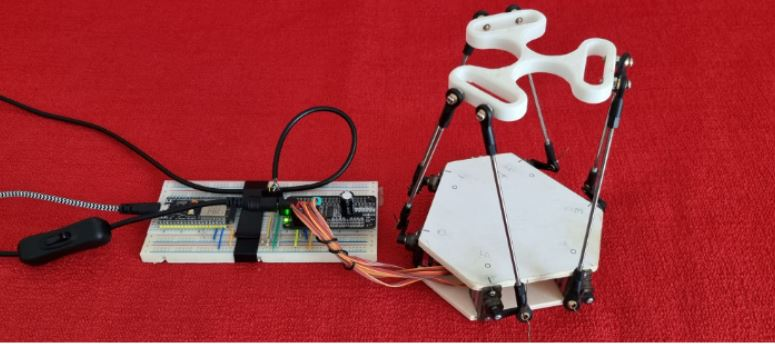
\includegraphics[width=\textwidth]{nicplatform2}
	\caption{Jeanmonod’s implementation of a single hexapod platform, physical model \cite{nicdoc}}
	\label{fig:nicplatform2}
\end{figure}

Jeanmonod's implementation would need to be modified to fit the goals of this thesis. The top and bottom platforms are different sizes, which would not work for a stacked hexapod platform where each level is of uniform size. Making each level the same size makes manufacturing and design much easier; however, the load on each level is not uniform, which means that the bottom-most level experiences much more force and wear than the top-most level. In future implementations of stacked hexapod platforms, a cascading design (where the bottom-most level is larger and has more powerful motors, and the size/weight of each platform decreases as the number of platforms increase) would be recommended.

The implementation for this thesis is shown below. It uses a common plate design which can be modified for the needs of each individual platform. The base plate of the first platform, Figure \ref{fig:firstbase}, has three through holes for 3/8”-16 bolts to attach the Fo-SHIP to a wooden base. The base plates of the second and fourth platform, Figure \ref{fig:secondbase}, have mounting slots for a PCA9685 servo driver and an MPU6050 IMU (details in Section \ref{ssec:2s5s2}). The base plate of the third platform, Figure \ref{fig:thirdbase}, has a mounting slot for the MPU6050 only. The middle plate of each platform, Figure \ref{fig:midbase}, has holes to allow servo wires to pass through (this plate sits on top of the servos). The top / end effector plate, Figure \ref{fig:endplate}, has mounting holes to attach the iSBL-SF array adapter. Figure \ref{fig:secondplatstack} shows the spacing between plates for the second platform. All plates were modeled using SOLIDWORKS.

\begin{figure}[htbp]
	\centering
	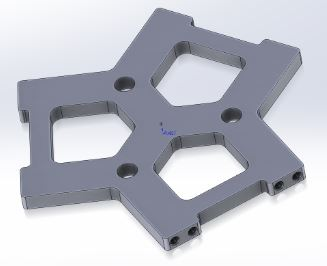
\includegraphics[width=0.5\textwidth]{firstbase}
	\caption{First platform base plate}
	\label{fig:firstbase}
\end{figure}

\begin{figure}[htbp]
	\centering
	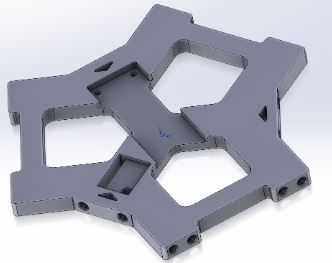
\includegraphics[width=0.5\textwidth]{secondbase}
	\caption{Second and fourth platform base plate}
	\label{fig:secondbase}
\end{figure}

\begin{figure}[htbp]
	\centering
	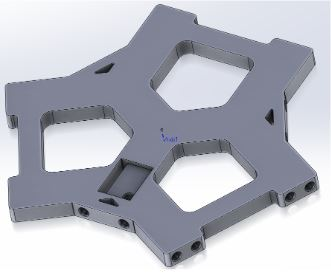
\includegraphics[width=0.5\textwidth]{thirdbase}
	\caption{Third platform base plate}
	\label{fig:thirdbase}
\end{figure}

\begin{figure}[htbp]
	\centering
	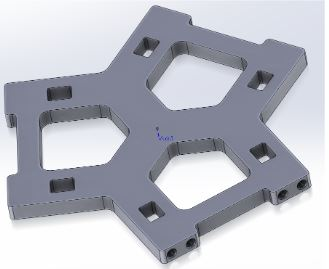
\includegraphics[width=0.5\textwidth]{midbase}
	\caption{Middle plate for all platforms}
	\label{fig:midbase}
\end{figure}

\begin{figure}[htbp]
	\centering
	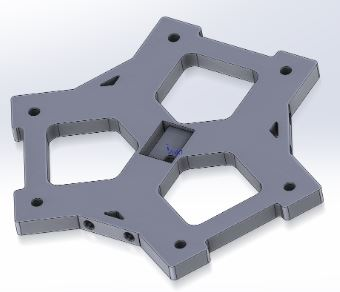
\includegraphics[width=0.5\textwidth]{endplate}
	\caption{End effector plate}
	\label{fig:endplate}
\end{figure}

\begin{figure}[htbp]
	\centering
	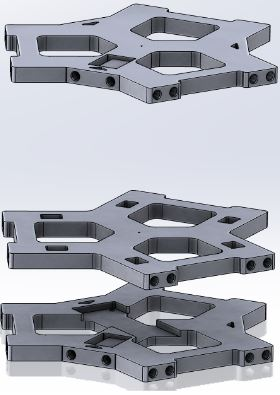
\includegraphics[width=0.5\textwidth]{secondplatstack}
	\caption{Spacing of plates for second platform}
	\label{fig:secondplatstack}
\end{figure}

The plates were printed in the Cal Poly Mustang ‘60 Machine Shop on Prusa Mk.3 FDM printers using blue PETG. PETG was chosen due to its strength, durability, non-brittle nature, and heat resistance when compared to materials like PLA \cite{plapetg}. Figure \ref{fig:rawpca} shows one of the printed base plates with a PCA9685 servo driver resting in its mounting slot.

\begin{figure}[htbp]
	\centering
	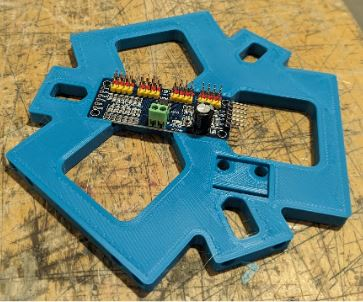
\includegraphics[width=0.5\textwidth]{rawpca}
	\caption{Printed base plate with PCA9685 servo driver}
	\label{fig:rawpca}
\end{figure}

A bill of materials for all components of the Fo-SHIP is shown in Table \ref{tab:bomfoship}. Note that some equipment used for fabrication, such as soldering irons and 3D printers, is essential to the build and is not factored into the bill of materials.

\begin{table}[htbp]
	\centering
	\caption{Bill of Materials for Fo-SHIP}
	\label{tab:bomfoship}
	\begin{tabular}{|c|c|c|c|}
		\hline
		Item & Quantity & Price (ea) & Vendor \\
		\hline
		Blue PETG filament, 1kg & 1 & \$25 & Amazon \\
		\hline
		MG996R servo motors, 6 pieces & 4 & \$27 & Amazon \\
		\hline
		Metal ball joint, M3, 12 pieces & 4 & \$12 & Amazon \\
		\hline
		Threaded inserts, M3, 120 pieces & 2 & \$7 & Amazon \\
		\hline
		Threaded rods, M3, 100mm, 12 pieces & 2 & \$6 & Amazon \\
		\hline
		Aluminum servo horns, M3, 10 pieces & 3 & \$14 & Amazon \\
		\hline
		M3x8 socket head cap screws, 100 pieces & 1 & \$8 & Amazon \\
		\hline
		M3x5 socket head cap screws, 50 pieces & 2 & \$5 & Amazon \\
		\hline
		M3 hexagonal nuts, 100 pieces & 1 & \$10 & Ace Hardware \\
		\hline
		M3x20 phillips head screws, 25 pieces & 1 & \$10 & Ace Hardware \\
		\hline
		3/8”-16 hexagonal bolt & 3 & \$1 & Ace Hardware \\
		\hline
		3/8”-16 hexagonal nut & 3 & \$1 & Ace Hardware \\
		\hline
		M2x4 screw, 5 pieces & 1 & \$2 & Ace Hardware \\
		\hline
		M2 hexagonal nut, 5 pieces & 1 & \$2 & Ace Hardware \\
		\hline
		ESP32-WROOM microcontroller & 1 & \$10 & Amazon \\
		\hline
		PCA9685 servo driver board, 2 pieces & 1 & \$14 & Amazon \\
		\hline
		MPU6050 IMU, 3 pieces & 2 & \$10 & Amazon \\
		\hline
		DC variable power supply, 0-30V, 0-30A & 1 & \$50 & Amazon \\
		\hline
		MPU6050 IMU, 3 pieces & 2 & \$10 & Amazon \\
		\hline
		Jumper wires, assorted & 2 & \$7 & Amazon \\
		\hline
		Solderless breadboard pack & 1 & \$8 & Amazon \\
		\hline
		24-gauge wire, assorted colors, 30 feet each & 1 & \$15 & Amazon \\
		\hline
		Scrap wood boards for base of platform & 2 & \$0 & Machine shop \\
		\hline
		\multicolumn{2}{|c|}{Total Cost} & \$292 &  \\
		\hline
	\end{tabular}
\end{table}

\vspace{2ex}
Lastly, Jeanmonod’s code implementation uses the dimensions of the platform to compute the inverse kinematics model. Certain parameters are used to perform these calculations; the values used for this thesis’s implementation (based on the models above) are located in Table \ref{tab:foshipparams}. A diagram of the parameters can be seen below in Figure \ref{fig:hexparams}.

\begin{table}[!htbp]
	\centering
	\caption{Parameters for hexapod platform code implementation}
	\label{tab:foshipparams}
	\renewcommand{\arraystretch}{1.2}
	\begin{tabular}{|>{\centering\arraybackslash}m{3cm}|>{\centering\arraybackslash}m{3cm}|>{\centering\arraybackslash}m{1.5cm}|>{\centering\arraybackslash}m{5cm}|}
		\hline
		\makecell{Parameter name} & \makecell{Measurement} & Units & \makecell{Determination method} \\
		\hline
		ROD\_LENGTH & 106.0 & mm & Measured six assembled threaded rods with ball joints attached, took average, then assembled all other rods and set to that uniform length \\
		\hline
		Z\_HOME & 100 & mm & Personal preference - servo horns are horizontal at 90mm, but setting to 100mm gives greater range-of-motion for angular displacement \\
		\hline
		ARM\_LENGTH & 24.0 & mm & Measured six aluminum servo horns with calipers, took average \\
		\hline
		THETA\_P & 50.02 & deg & Computed from CAD model, verified using calipers and trigonometry on printed parts \\
		\hline
		THETA\_B & 20.53 & deg & Computed from CAD model, verified using calipers and trigonometry on printed parts \\
		\hline
		THETA\_S & 120 & deg & Computed from CAD model, verified using calipers and trigonometry on printed parts \\
		\hline
		P\_RAD & 57.73 & mm & Computed from CAD model, verified using calipers on assembled platform, took average of three readings \\
		\hline
		B\_RAD & 82.7 & mm & Computed from CAD model, verified using calipers on assembled platform, took average of three readings \\
		\hline
	\end{tabular}
\end{table}

\begin{figure}[!htbp]
	\centering
	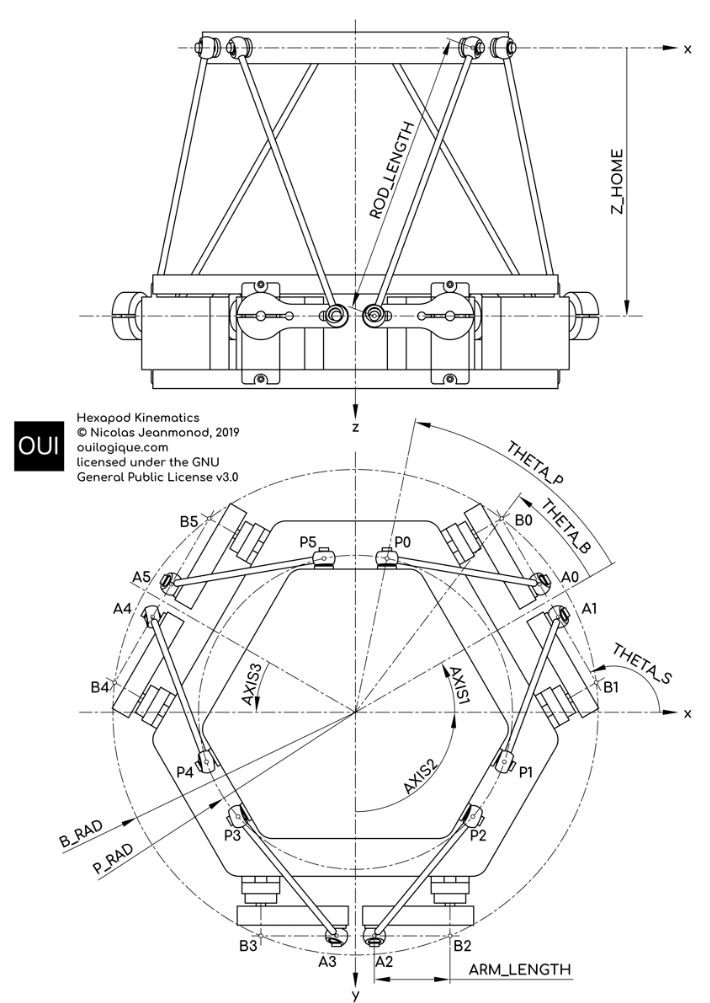
\includegraphics[width=0.9\textwidth]{hexparams}
	\caption{Parameters for hexapod platform in Jeanmonod’s code implementation \cite{nichub}}
	\label{fig:hexparams}
\end{figure}

\vspace{10pt}
\section{Electrical Design} \label{sec:2s3}
The electrical wiring and design of the Fo-SHIP is relatively straightforward - it consists of an ESP32 microcontroller communicating with two PCA9685 servo drivers and five MPU6050 IMUs. The PCA9685 is a servo controller board that communicates with a microcontroller (or other controller) over I\textsuperscript{2}C, a common electronics protocol. It has 16 channels that use standard hobby servo motor wiring (ground / 5V / PWM); by sending the correct message over I\textsuperscript{2}C, the microcontroller can control up to 16 servo motors, LEDs, or anything that takes in a PWM signal \cite{pca9685datasheet}.

PWM, or pulse width modulation, is a technique for modulating the width of an electrical pulse. For servo motors, a common protocol is to divide pulses into 20ms periods and set the output to “high” for a certain amount of time, depending on the angle desired. Figure 16 shows a common configuration for hobby servo motors. The specifics of how the instructions for a certain pulse width are sent from the microcontroller to the PCA9685 are explained in section 2.5.

\begin{figure}[htbp]
	\centering
	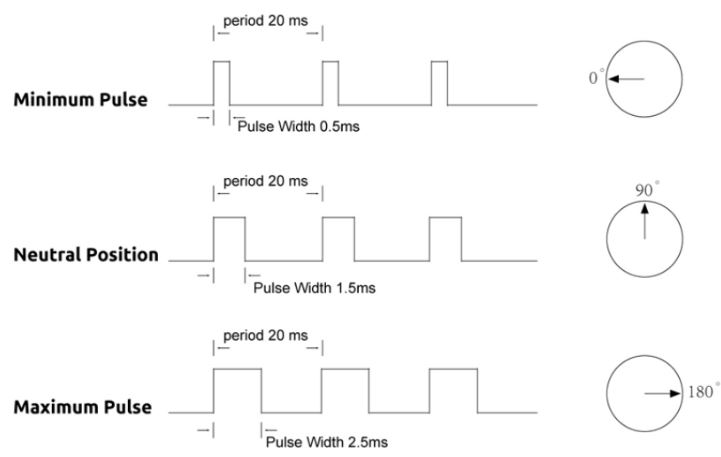
\includegraphics[width=0.9\textwidth]{servotiming}
	\caption{Hobby servo motor PWM timing \cite{servos}}
	\label{fig:servotiming}
\end{figure}

The MPU6050s also communicate over the same I\textsuperscript{2}C line. Each MPU6050 reads linear acceleration and angular velocity about three axes (XYZ). There is one MPU6050 attached to the wooden base of the Fo-SHIP, and one attached to the top of each hexapod platform. When the Fo-SHIP is at rest, the acceleration values can be read and converted to a 3D orientation. Using this data, any “slop” in the system is accounted for - if the Fo-SHIP’s end effector is set to 15° about the X axis, the true orientation for each hexapod platform can be measured (and it can be confirmed if the end effector is actually oriented at 15°). The specifics of how data is sent between the MPU6050s and the ESP32 microcontroller, how the accelerometer data is converted to orientation, and how the true orientation can be used to correct the forward kinematics model of the Fo-SHIP are discussed in Section \ref{sec:2s5}. 

For I\textsuperscript{2}C, all that is needed is four wires: ground, power, SDA (data), and SCL (clock). For two (or more) devices that are communicating over I\textsuperscript{2}C, all devices share the same line for each of the four wires, and a pullup resistor is added to the SDA and SCL lines. Figure \ref{fig:i2cwiring} shows a common wiring schematic for I\textsuperscript{2}C communication.

\begin{figure}[htbp]
	\centering
	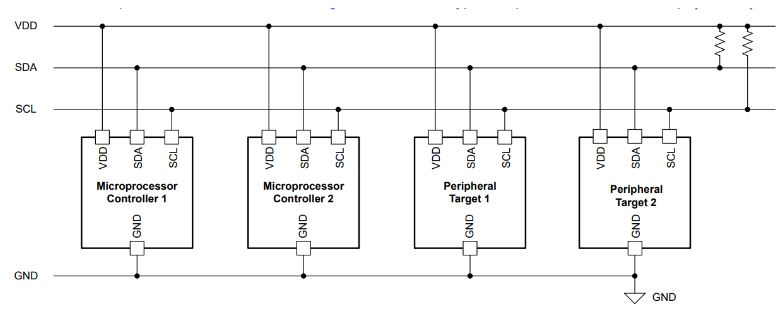
\includegraphics[width=0.9\textwidth]{i2cwiring}
	\caption{Typical I\textsuperscript{2}C wiring \cite{tiI2C}}
	\label{fig:i2cwiring}
\end{figure}

The ESP32, PCA9685s, and MPU6050s are all connected to the same I\textsuperscript{2}C bus. Each MPU6050 has an AD0 pin that must be pulled low (to ground) to choose which IMU to read from. Additionally, the ESP32 is connected via USB to a laptop, providing logic power and facilitating data transfer via UART. There is a button connected to one of the ESP32 general purpose input-output (GPIO) pins for user interaction and to begin data collection. The ESP32 is also connected to an STM32 microcontroller via a serial bus (RX/TX). Lastly, the PCA9685s have an additional power input to provide high-current power to the 24 servos of the Fo-SHIP. A wiring diagram for the Fo-SHIP can be seen in Figure \ref{fig:foshipwiring}.

\begin{figure}[htbp]
	\centering
	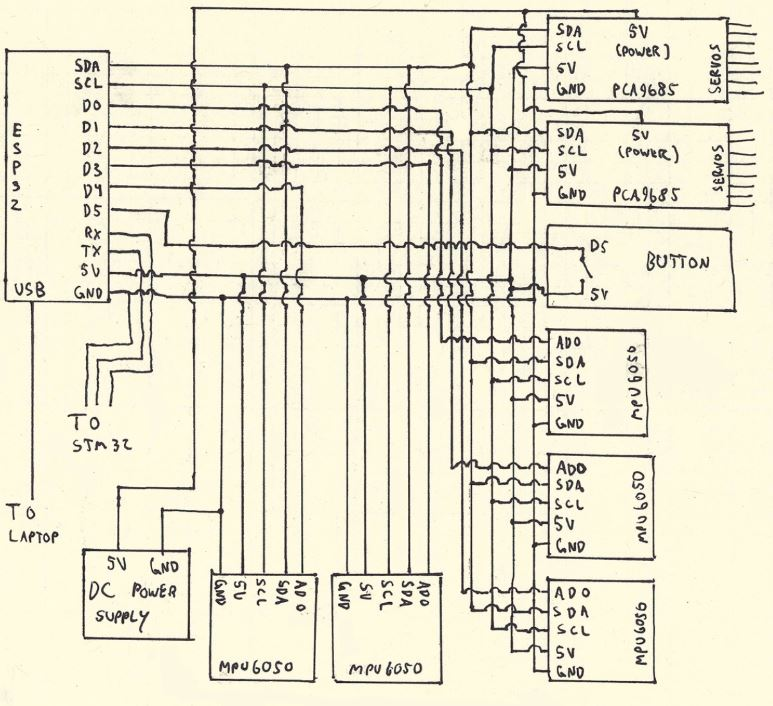
\includegraphics[width=0.9\textwidth]{foshipwiring}
	\caption{Fo-SHIP wiring diagram}
	\label{fig:foshipwiring}
\end{figure}

\section{Manufacturing and Assembly} \label{sec:2s4}
As stated in Section \ref{sec:2s2}, the plates of the Fo-SHIP were printed in the Cal Poly Mustang ‘60 Machine Shop over the course of two weeks. M3 threaded inserts were heat-set into blind and through holes in the plates using a soldering iron. Note that the mounting slots for the PCA9685 and MPU6050 have through holes for heat-set inserts as well.

A wooden base was manufactured from two boards: one on the bottom that has a large circular cutout, and another on top that has through holes for the mounting bolts. The bottom board is necessary to provide an offset between the ground and the mounting bolts and nuts. The wooden base can be seen in Figure \ref{fig:woodenbase}.

\begin{figure}[htbp]
	\centering
	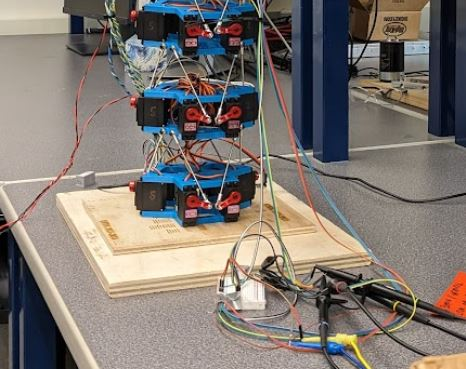
\includegraphics[width=0.9\textwidth]{woodenbase}
	\caption{Wooden base of Fo-SHIP}
	\label{fig:woodenbase}
\end{figure}

The Fo-SHIP was assembled one level at a time, starting with the bottom platform. The servos were mounted between the base and middle plate of the first platform, loosely secured using M3x5 socket head cap screws. The servos were adjusted to be parallel with the edges of the plates, and the screws ere tightened in a star pattern to avoid uneven clamping forces and misalignments. The servos were then powered and set to an angle of 90° (horizontal). Aluminum servo horns were placed on the servo output; adjacent horns were placed to be pointed towards each other as shown in Figure \ref{fig:firsttwoplat}. The horns were attached using screws to the servo output and were further secured via small, off-center screws that clamp the body of the horn around the servo output.

The threaded rod linkages were assembled by screwing on threaded ball joint connectors at both ends, turning each connector an equal amount to ensure equal thread penetration. The length between the centers of each ball joint bearing was measured, and the ball joints were adjusted until the length is 106mm ± 1mm. For each platform, six linkages were gathered and each was attached to the inside of a servo horn at the furthest threaded hole. An M3x20 screw was placed through the ball joint bearing and screwed into the servo horn. Once tightened, an M3 nut was secured to the end of the M3x20 screw and torqued to prevent the connection from loosening.

A second platform was assembled as described in the previous paragraph up until after the servo horns were secured. Then, both platforms were laid horizontally on a table and the linkages from the first platform were secured to the corresponding threaded inserts on the base of the second platform using M3x8 screws. Care was taken to avoid over-torquing any threaded inserts, since they are secured only by melted plastic. 

The above process was repeated until four platforms had been assembled. At this point, the end effector plate was attached to the top-most platform.

\begin{figure}[htbp]
	\centering
	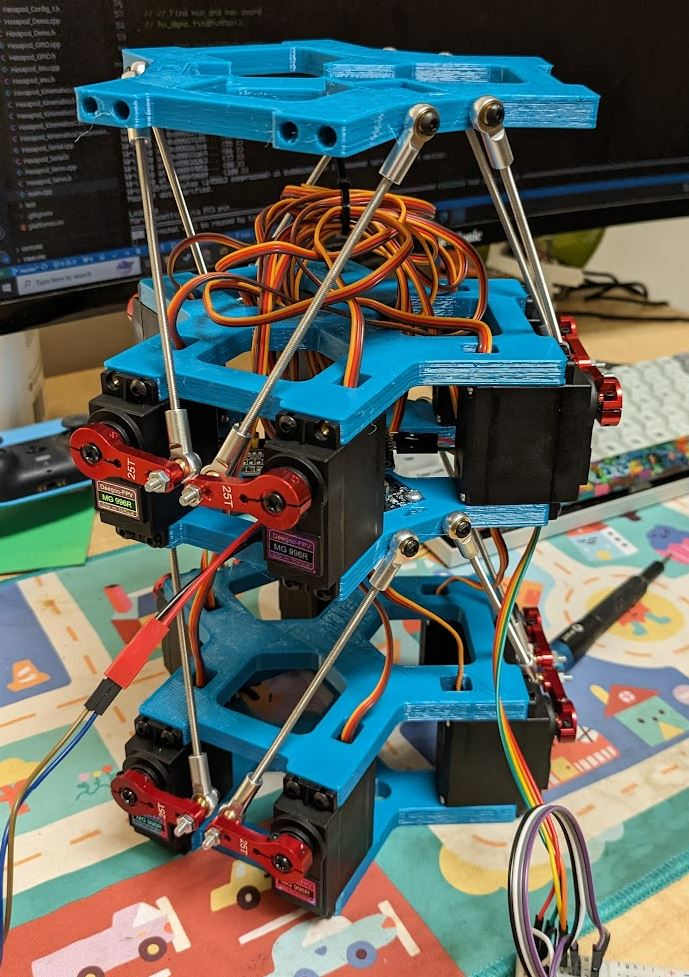
\includegraphics[width=0.9\textwidth]{firsttwoplat}
	\caption{Assembled Fo-SHIP, first two layers}
	\label{fig:firsttwoplat}
\end{figure}

Once all platforms were assembled, an MPU6050 was attached to the base of each platform (besides the first level), to the end effector plate, and to the wooden base. The MPU6050s were secured using M3x5 screws and care was taken to avoid over-torquing the screws and deforming the plastic beneath, which would result in an altered angle reading from the IMUs. Then, the PCA9685 boards were attached to the base of the second and fourth platform and secured with M2x4 screws and M2 nuts. Once secured, the servo wires were attached to the PCA9685 boards in a clockwise pattern. A number was written on each servo’s body to note which pins it connects to on its corresponding PCA9685 board. Wires were added to each MPU6050 and PCA9685 in accordance with the wiring diagram in Section \ref{sec:2s3} and were connected to a breadboard that held the ESP32 microcontroller. 

The breadboard and the button included in the wiring diagram were secured to the wooden base with adhesive. Loose wires were joined using cable ties, and hot glue was used to insulate electrical connections and prevent wires from dislodging from the breadboard. The fully-assembled Fo-SHIP with all platforms and wiring can be seen in Figure \ref{fig:fullplats} below.

\begin{figure}[htbp]
	\centering
	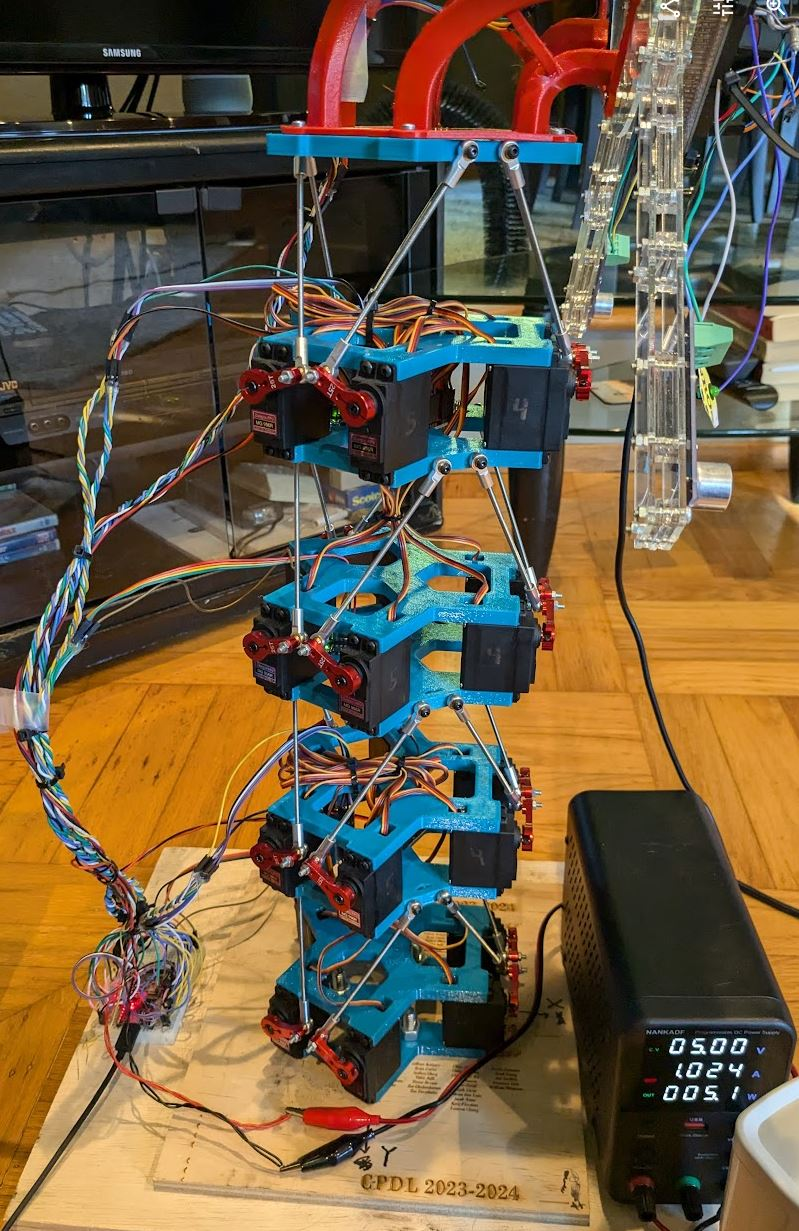
\includegraphics[width=0.9\textwidth]{fullplats}
	\caption{Assembled Fo-SHIP, first two layers}
	\label{fig:fullplats}
\end{figure}

\vspace{10pt}
\section{Software Design} \label{sec:2s5}
The code running on the ESP32 to control the Fo-SHIP is quite complex and has many different functions and files. This section will be broken down into six subsections. The first will show custom structs used for the code and the configuration / parameters of each platform of the Fo-SHIP. The second will discuss the MPU6050 failures and how a workaround was implemented. The third will discuss the main program initialization and loop, and will include a finite-state machine representation of the code. The fourth will detail the forward kinematics calculations for the multi-platform configuration, focusing on the big-picture of how one platform affects the next. The fifth will derive the inverse kinematics algorithm used to calculate servo angles for a single platform’s setpoint. The last will explain some demonstration functions that show the full range-of-motion of the Fo-SHIP.

As stated previously, the majority of this code is built off of Nicolas Jeanmonod’s implementation on GitHub \cite{nichub}, and the Fo-SHIP would not be functional without his contributions.

\subsection{Custom Structs and Hexapod Configuration} \label{ssec:2s5s1}
The Fo-SHIP uses a few custom structs for its data processing. First, \verb|calibration_t| is a struct used for saving the gains and offsets of each individual servo. 

\begin{lstlisting}[language=C++]
typedef struct
{
	double gain;
	int offset;
} calibration_t;
\end{lstlisting}

Next, \verb|angle_t| is a struct used for saving information about each servo’s angle in a variety of units: radians, degrees, microseconds (for PWM) and PWM value (int from 0 to 4096).

\begin{lstlisting}[language=C++]
typedef struct
{
	double rad;			// Servo angle in radian.
	double deg;			// Servo angle in degrees.
	int us;				// Servo angle in us (PWM).
	uint16_t pwm_us; 	// Servo angle in range 0 to 4096 (PWM).
	double debug;		// Used for debug.
} angle_t;
\end{lstlisting}

Lastly, \verb|platform_t| is the most common struct used in the main program code. It defines the setpoint for a single platform with six coordinates, one for each major axis: (X, Y, Z, A, B, C), where A is roll about the X axis, B is pitch about the Y axis, and C is yaw about the Z axis.

\begin{lstlisting}[language=C++]
typedef struct
{
	double hx_x; // Surge, translation along X axis (mm)
	double hx_y; // Sway, translation along Y axis (mm)
	double hx_z; // Heave, translation along Z axis (mm)
	double hx_a; // Roll, rotation around X axis (rad)
	double hx_b; // Pitch, rotation around Y axis (rad)
	double hx_c; // Yaw, rotation around Z axis (rad)
} platform_t;
\end{lstlisting}

Many configuration parameters are stored in \verb|Hexapod_Config1.h|. These include the parameters in Table \ref{tab:foshipparams}, as well as offset values for each servo, the full range of a servo described with a pulse width timing, minimum and maximum values for each axis of motion, and the orientation of each servo relative to the coordinate system.

\subsection{MPU6050 Failure and Workaround} \label{ssec:2s5s2}
After fully assembling the Fo-SHIP, it was discovered that only one out of the six MPU6050s purchased from Amazon was functional. Due to a limited budget and limited time (and after much testing of the MPU6050s to determine if they were truly faulty or if it was a code issue, which it was not), it was decided to forgo using any of the MPU6050s for orientation correction. However, the amount of slop in the Fo-SHIP’s many platforms required some sort of orientation correction for the forward kinematics calculations. 

Thankfully, the iSBL receiver array has a higher quality (and functional) IMU which outputs the orientation of the end effector, which will be discussed more in Chapter 4. As a workaround, at the time of processing an acoustic measurement, the current orientation of the end effector is sent over UART from the STM32 to the ESP32. This orientation is assumed to be the true orientation of the end effector (top-most platform’s top plate). Assuming that the amount of slop in the system is uniform for each platform, the true orientation of a single platform relative to the one beneath it can be estimated as shown:

\begin{lstlisting}[language=C++]
modPos = currentPos;
modPos.hx_a = radians(stm_roll/4);
modPos.hx_b = radians(stm_pitch/4);
modPos.hx_c = radians(stm_yaw/4);
getEndEffectorCoords(&modPos, &modPos, &modPos, &modPos, false);
\end{lstlisting}

While this may seem like a large simplification, it improves the accuracy of the Fo-SHIP’s position estimate by over 100\%. 

The original implementation of the MPU6050s is still in the code and will be explained here. The workflow for extracting the angle of each platform relative to the one beneath it using the MPU6050s is below. This workflow is for a single MPU6050 and is repeated for each platform's IMU:

\begin{itemize}[noitemsep,topsep=0pt]
	\item Take a number of readings from the MPU6050’s accelerometer, communicating over I\textsuperscript{2}C, and take the average to reject noise
	\item Convert the acceleration data into Euler angles (absolute orientation)
	\item Convert the absolute Euler angles into a rotation matrix
	\item Take the transpose of this matrix
	\item Multiply the absolute rotation matrix for this platform by the transpose of the rotation matrix of the platform beneath it to get the relative orientation rotation matrix for this platform
	\item Extract the relative Euler angles for this platform from the relative orientation rotation matrix
	\item Save these Euler angles as the relative orientation of each platform
\end{itemize}

\noindent In the \verb|main.cpp| file, see these functions for more details:

\begin{itemize}[noitemsep,topsep=0pt]
	\item \verb|void readMPU(int IMU_NUM, int num_avgs);|
	\item \verb|void getEulerFromMPU(float *IMU_AccelData, float *IMU_Angles);|
	\item \verb|void getRotMatFromEuler(float *IMU_Angles, float *IMU_RotMat);|
	\item \verb|void getEulerFromRotMat(float *IMU_RotMat, float *IMU_Angles);|
	\item \verb|void multiply3x3Matrices(float *matA, float *matB, float|\\ \verb|*result);|
	\item \verb|void transposeMatrix(float *mat, float *result);|
	\item \verb|void multiply3x3MatrixVector(float *mat, float *vec, float|\\ \verb|*result);|
\end{itemize}

\subsection{Main Program} \label{ssec:2s5s3}
The main program in \verb|main.cpp| does a few things: it starts and maintains a serial connection with the STM32 and the laptop for data collection; it reads from the MPU6050s and computes their relative orientation; it controls the motion of each platform of the Fo-SHIP; and it performs the forward kinematics calculations that provide the ground-truth position estimate for the iSBL array, arguably its most important role. A finite-state machine representation of the \verb|main.cpp| code can be seen below.

\begin{figure}[htbp]
	\centering
	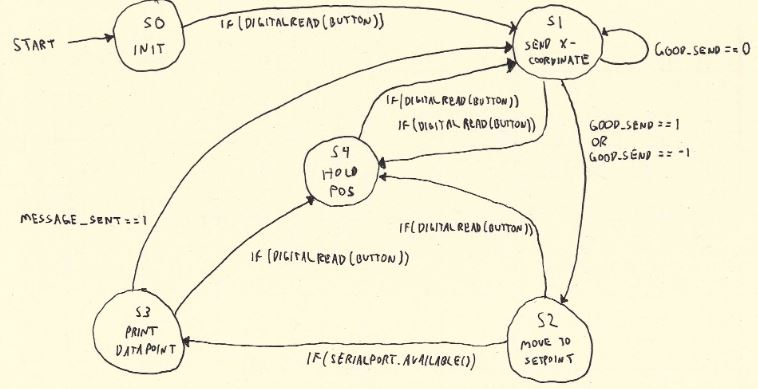
\includegraphics[width=0.9\textwidth]{foshipfsm}
	\caption{Finite-state machine diagram for Fo-SHIP code}
	\label{fig:foshipfsm}
\end{figure}

\noindent In the initialization state, the program does the following:

\begin{itemize}[noitemsep,topsep=0pt]
	\item Initializes the GPIO pins for each MPU6050 and the input button
	\item Begins the serial connection with the STM32 and the laptop
	\item Initializes the MPU6050s, setting their sensitivity and data rates
	\item Makes the top platform pitch forward and backward to show that the system is working
	\item Performs any demonstration functions if they are selected (see Section \ref{ssec:2s5s6})
\end{itemize}

After this, it waits until the button is pressed before entering the main loop. This gives time for the iSBL array to initialize and get an initial orientation.

Once the button is pressed and the main loop begins, the following sequence repeats until the button is pressed again (in which case, it pauses and restarts the loop). This sequence is meant for data collection - for a fixed transmitter location, the Fo-SHIP will move through a variety of points and record the position estimate from the STM32 and the iSBL-SF algorithm, then compare it to the true position as estimated by the Fo-SHIP. The loop executes the following steps:

\begin{itemize}[noitemsep,topsep=0pt]
	\item Calculates the axes that it should iterate through (XYZ or ABC)
	\item For each axis to iterate through, it does the following:
	
	\begin{itemize}[noitemsep,topsep=3ex]
		\item Based on the next setpoint of the Fo-SHIP, sends the x-coordinate of the iSBL array's center to the STM32
		\item Moves to the next setpoint for that axis (for example, moves from X = 5mm to X = 4mm)
		\item Waits while the iSBL-SF algorithm calculates a position estimate based on acoustic readings for the current setpoint
		\item Prints a datapoint to the laptop's serial connection containing multiple position estimates from the iSBL-SF algorithm, and the true position of the platform as calculated by the Fo-SHIP
		\item Repeats from the top of this list until all setpoints for a given axis have been tested (for example, testing all points between X = 20mm and X = -20mm)
	\end{itemize}
\end{itemize}

First, the Fo-SHIP calculates which axes it is going to test for this loop. In testing, it was found helpful to sometimes only test the linear (XYZ) axes, and sometimes only test the rotational (ABC) axes. For the final testing, all axes were tested and a flip-flop variable was assigned so that all axes were tested equally. 

\begin{lstlisting}[language=C++]
bool translational_axes = false;
...
if (translational_axes) 
{
	axes[0] = "X";
	axes[1] = "Y";
	axes[2] = "Z";
}
else 
{
	axes[0] = "Z";
	axes[1] = "B";
	axes[2] = "C";
}
\end{lstlisting}

The maximum and minimum values of each axis, as well as the step size increment, are defined in the main loop.

\begin{lstlisting}[language=C++]
if (axes[axis] == "X") {
	start_val = 5;
	end_val = -5;
	step_increment = linear_step_increment;
...
} else if (axes[axis] == "A") {
	start_val = radians(5);
	end_val = radians(-5);
	step_increment = angular_step_increment;
...
\end{lstlisting}
	
Then, each axis is tested individually. First, the new position of the platform is calculated, and true orientation compensation is applied as described in Section \ref{ssec:2s5s2}. The Fo-SHIP calculates what the next x-coordinate of the iSBL array’s center will be after this new move is executed. While it would be more accurate to move first, get the new orientation, and use that as the platform’s true position, this approach is preferred. It is easier to implement, is more reliable (don’t have to wait for the IMU to stabilize for its new setpoint), works better timing-wise, and is accurate enough for testing purposes. 

\begin{lstlisting}[language=C++]
for (float current_val = start_val*(1-stationary); current_val >= end_val; current_val -= step_increment*(1-stationary)) {
	platform_t newPos = {0, 0, 0, 0, 0, 0};
	
	if (axes[axis] == "X") newPos.hx_x = current_val;
	else if (axes[axis] == "Y") newPos.hx_y = current_val;
	else if (axes[axis] == "Z") newPos.hx_z = current_val;
	else if (axes[axis] == "A") newPos.hx_a = current_val;
	else if (axes[axis] == "B") newPos.hx_b = current_val;
	else if (axes[axis] == "C") newPos.hx_c = current_val;
	...
	platform_t modPos = newPos;
	float rollDiff = modPos.hx_a - currentPos.hx_a;
	float pitchDiff = modPos.hx_b - currentPos.hx_b;
	float yawDiff = modPos.hx_c - currentPos.hx_c;
	modPos.hx_a = radians(stm_roll/4) + rollDiff;
	modPos.hx_b = radians(stm_pitch/4) + pitchDiff;
	modPos.hx_c = radians(stm_yaw/4) + yawDiff;
	...
	getEndEffectorCoords(&modPos, &modPos, &modPos, &modPos, false);
	...
	float next_val = true_x / 1000;
\end{lstlisting}

The reason for sending the x-coordinate is covered more in Chapter 3, but it is necessary for proving a simulated “depth” measurement for the iSBL-SF algorithm. In the full underwater application, a pressure sensor would provide a depth measurement, which is essential for the iSBL-SF algorithm to work properly with short baselines. Since pressure sensors would not work for the above-water testing here, the true x-coordinate of the iSBL array is sent to the STM32 and is used for depth measurement simulation.

Next, a custom function \verb|sendRobustFloat()| is used to ensure that the \verb|true_x| value is sent to the STM32. The function uses checksums and start/end characters to ensure robust data transmission. Initially, there were many unexpected issues with sending data to the STM32 from the ESP32 (but not the other way around), which may suggest a faulty TX-to-RX wire. This function is called up to three times; once a message is sent, if the checksum calculated by the STM32 does not match the one sent by the ESP32, the STM32 instructs the ESP32 to send a message again. If this fails three times, the datapoint is skipped.

\begin{lstlisting}[language=C++]
void sendRobustFloat(float value) {
	char message[50];
	int messageLength = snprintf(message, sizeof(message), "%.4f", value);
	
	int checksum = 0;
	for (int i = 0; i < messageLength; i++) {
		checksum += message[i];
	}
	checksum %= CHECKSUM_MODULUS;
	
	SerialPort.print(START_MARKER);
	SerialPort.print(message);
	SerialPort.print(',');
	SerialPort.print(checksum);
	SerialPort.print(END_MARKER);
	SerialPort.println();
	
	// ensure transmission is complete
	SerialPort.flush();
}
\end{lstlisting}

Multiple times in the code, a blocking \verb|while()| loop is used. A block similar to the one below is used to allow the button press to be registered (to reset the data collection or pause it) when a blocking function is necessary.

\begin{lstlisting}[language=C++]
while (!SerialPort.available()){
	
	// if the button is pressed,
	if (digitalRead(BUTTON)){
		
		// turn the LED on
		digitalWrite(LED, HIGH);
		
		// move back to home
		moveSlowly(&currentPos, &home_coords[0], 20, binaryToDecimal(move_str));
		currentPos = {0, 0, 0, 0, 0, 0};
		
		// break out of all the loops
		shouldBreak = true;
		
		// turn the LED back off
		digitalWrite(LED, LOW);
		Serial.println("BUTTON PRESSED, 1");
		
		// wait until the button is pressed again to resume testing
		while (!digitalRead(BUTTON)){}
		digitalWrite(LED, HIGH);
		delay(1000);
		break;
	}
}
\end{lstlisting}

Once the next x-coordinate is sent, the Fo-SHIP executes the move to the next setpoint. Depending on the type of test being run (gradual or rapid movement), the Fo-SHIP moves at a different speed. Every movement uses the custom \verb|moveSlowly()| function, which linearly interpolates between the current setpoint and the desired (next) setpoint. Notably, the function moves each platform to the same setpoint - it would need to be modified to control each platform individually.

\begin{lstlisting}[language=C++]
void moveSlowly(platform_t *startCoords, platform_t *endCoords, uint16_t num_steps, uint8_t which_platform) {
	platform_t startPos = *startCoords;
	platform_t endPos = *endCoords;
	int8_t movOK = -1;
	
	for (uint16_t step = 0; step < num_steps; step++) {
		double t = ((double)step) / (double)num_steps;
		
		// linearly interpolate between startPos and endPos
		platform_t interpPos;
		interpPos.hx_x = startPos.hx_x + t * (endPos.hx_x - startPos.hx_x);
		interpPos.hx_y = startPos.hx_y + t * (endPos.hx_y - startPos.hx_y);
		interpPos.hx_z = startPos.hx_z + t * (endPos.hx_z - startPos.hx_z);
		interpPos.hx_a = startPos.hx_a + t * (endPos.hx_a - startPos.hx_a);
		interpPos.hx_b = startPos.hx_b + t * (endPos.hx_b - startPos.hx_b);
		interpPos.hx_c = startPos.hx_c + t * (endPos.hx_c - startPos.hx_c);
		
		// calculate servo angles using the interpolated positions
		movOK = 0;
		if (which_platform & (1 << 3)) movOK += hx_servo.calcServoAngles(interpPos, servo_angles0, 0);
		if (which_platform & (1 << 2)) movOK += hx_servo.calcServoAngles(interpPos, servo_angles1, 1);
		if (which_platform & (1 << 1)) movOK += hx_servo.calcServoAngles(interpPos, servo_angles2, 2);
		if (which_platform & (1 << 0)) movOK += hx_servo.calcServoAngles(interpPos, servo_angles3, 3);
		
		hx_servo.updateServos(movOK);
		
		delay(50);
	}
	
	// move to the final position
	movOK = 0;
	if (which_platform & (1 << 3)) movOK += hx_servo.calcServoAngles(endPos, servo_angles0, 0);
	if (which_platform & (1 << 2)) movOK += hx_servo.calcServoAngles(endPos, servo_angles1, 1);
	if (which_platform & (1 << 1)) movOK += hx_servo.calcServoAngles(endPos, servo_angles2, 2);
	if (which_platform & (1 << 0)) movOK += hx_servo.calcServoAngles(endPos, servo_angles3, 3);
	hx_servo.updateServos(movOK);
}
\end{lstlisting}

Once the Fo-SHIP moves to its new position, it waits while the iSBL array records an acoustic pulse and the STM32 calculates new position estimates. Once the STM32 sends its results over, the ESP32 decodes the serial string, parses the information, and prints the important results to the laptop via serial. Notably, the ESP32 also includes the true position of the iSBL array, which the STM32 does not have access to for its calculations (besides the x-coordinate).

\begin{lstlisting}[language=C++]
String readSerialString() {
	String receivedString = "";
	while (SerialPort.available()) {
		char c = SerialPort.read();
		if (c == '\r' || c == '\n') {
			break;
		}
		receivedString += c;
		delay(2);
	}
	receivedString.trim();
	return receivedString;
}
// once the STM32 sends its data, parse it and put the data into floats
String receivedString = readSerialString();
float x_kf, y_kf, z_kf, x_r_isbl, y_r_isbl, z_r_isbl, x_isbl, y_isbl, z_isbl;
sscanf(receivedString.c_str(), "%f,%f,%f,%f,%f,%f,%f,%f,%f,%f,%f,%f", 
&x_kf, &y_kf, &z_kf, &x_r_isbl, &y_r_isbl, &z_r_isbl, 
&x_isbl, &y_isbl, &z_isbl, &stm_roll, &stm_pitch, &stm_yaw);

// once we have the new orientation of the platform, use it to recalculate the true end effector pos
modPos = currentPos;
modPos.hx_a = radians(stm_roll/4);
modPos.hx_b = radians(stm_pitch/4);
modPos.hx_c = radians(stm_yaw/4);
getEndEffectorCoords(&modPos, &modPos, &modPos, &modPos, false);

// since XYZ and ABC have different units, we need to format the current value differently
float printval;
printval = degrees(current_val*4);
if (translational_axes) printval = current_val*4;

// print a single datapoint / row
Serial.println(String(axes[axis]) + ", " + String(printval)+ ": "
+ String(x_kf) + ", " + String(y_kf) + ", " + String(z_kf) + "; " 
+ String(x_r_isbl) + ", " + String(y_r_isbl) + ", " + String(z_r_isbl) + "; "
+ String(x_isbl) + ", " + String(y_isbl) + ", " + String(z_isbl) + "; "
+ String(true_x) + ", " + String(true_y) + ", " + String(true_z) + "; "
+ String(stm_roll) + ", " + String(stm_pitch) + ", " + String(stm_yaw) + ";");
\end{lstlisting}

This process repeats until all values in an axis have been tested. Then, the next axis is tested until all three axes for that loop are iterated through. Then, the int \verb|translational_axes| flips its value and the other three axes are tested.

There is additional code for transmitting large chunks of data (like the entire \verb|adc_buf| data, as described in Chapter 3), but it is currently commented out.

\subsection{Multi-Platform Forward Kinematics Calculations} \label{ssec:2s5s4}
Similar to the deep reinforcement learning implementation in Section \ref{ssec:2s1s2}, the large-scale forward kinematics model assumes that each platform can be represented by two vectors: a translational vector defining the distance from the center of the base of a platform to the center of the top of a platform, and a rotational vector defining the vector normal to the top of the platform. Additionally, each platform has a constant offset in its local Z coordinate to account for the height of the servos. Figure \ref{fig:forwardkine} below shows the forward kinematics model in two dimensions, but the math scales to three dimensions.

In the diagram, there are some items to note. First, the Z axis is pointing in the opposite direction to the final implementation. Next, we work from the base up to the top, applying the previous rotation matrix to each subsequent level. Point xP denotes the center of the iSBL array, which has a constant offset vector which is rigidly attached to the top platform’s end effector. Each rotation matrix (R1, R3, etc.) is defined relative to the platform beneath it, not to the global frame - the second platform’s base’s rotation in the global frame is described by R2*R1*R0, but its rotation relative to the platform beneath it is just R2.

\begin{figure}[!htbp]
	\centering
	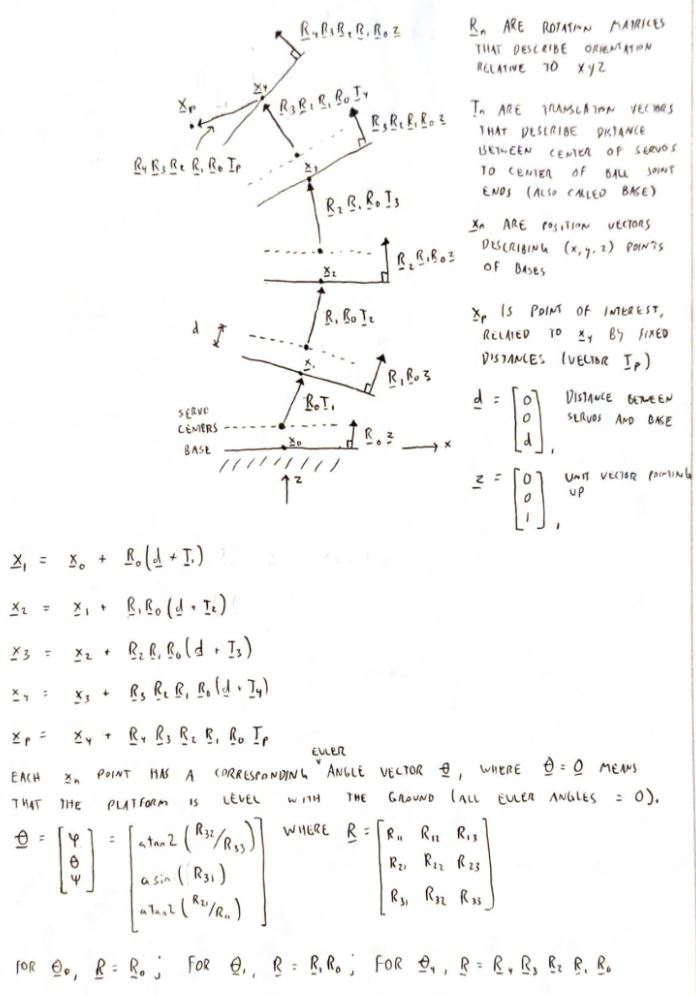
\includegraphics[width=0.9\textwidth]{forwardkine}
	\caption{Forward kinematics diagram}
	\label{fig:forwardkine}
\end{figure}

This forward kinematics model was implemented in the main code of the Fo-SHIP with the function below. The values \verb|true_x|, \verb|true_y|, and \verb|true_z| are then accessible by the rest of the program when needed.

\begin{lstlisting}[language=C++]
void getEndEffectorCoords(platform_t *coords1, platform_t *coords2, platform_t *coords3, platform_t *coords4, bool USE_IMU){
	float d[3] = {0, 0, -34};
	float TP[3] = {80 + 30, 0, -78.38 - 4};
	float zhome = static_cast<float>(Z_HOME);
	
	float T1[3] = {static_cast<float>(coords1->hx_x), static_cast<float>(coords1->hx_y), static_cast<float>(coords1->hx_z) + zhome};
	float T2[3] = {static_cast<float>(coords2->hx_x), static_cast<float>(coords2->hx_y), static_cast<float>(coords2->hx_z) + zhome};
	float T3[3] = {static_cast<float>(coords3->hx_x), static_cast<float>(coords3->hx_y), static_cast<float>(coords3->hx_z) + zhome};
	float T4[3] = {static_cast<float>(coords4->hx_x), static_cast<float>(coords4->hx_y), static_cast<float>(coords4->hx_z) + zhome};
	
	float eul1[3] = {0, 0, static_cast<float>(coords1->hx_c)};
	float eul2[3] = {0, 0, static_cast<float>(coords2->hx_c)};
	float eul3[3] = {0, 0, static_cast<float>(coords3->hx_c)};
	float eul4[3] = {0, 0, static_cast<float>(coords4->hx_c)};
	
	if (USE_IMU) {
		eul1[0] = IMU1_Angles[0];
		eul1[1] = IMU1_Angles[1];
		eul2[0] = IMU2_Angles[0];
		eul2[1] = IMU2_Angles[1];
		eul3[0] = IMU3_Angles[0];
		eul3[1] = IMU3_Angles[1];
		eul4[0] = IMU4_Angles[0];
		eul4[1] = IMU4_Angles[1];
	} else {
		eul1[0] = static_cast<float>(coords1->hx_a);
		eul1[1] = static_cast<float>(coords1->hx_b);
		eul2[0] = static_cast<float>(coords2->hx_a);
		eul2[1] = static_cast<float>(coords2->hx_b);
		eul3[0] = static_cast<float>(coords3->hx_a);
		eul3[1] = static_cast<float>(coords3->hx_b);
		eul4[0] = static_cast<float>(coords4->hx_a);
		eul4[1] = static_cast<float>(coords4->hx_b);
	}
	
	float R0[9] = {1, 0, 0, 0, 1, 0, 0, 0, 1};
	float R1[9] = {1, 0, 0, 0, 1, 0, 0, 0, 1};
	float R2[9] = {1, 0, 0, 0, 1, 0, 0, 0, 1};
	float R3[9] = {1, 0, 0, 0, 1, 0, 0, 0, 1};
	float R4[9] = {1, 0, 0, 0, 1, 0, 0, 0, 1};
	
	float R1R0[9] = {1, 0, 0, 0, 1, 0, 0, 0, 1};
	float R2R1R0[9] = {1, 0, 0, 0, 1, 0, 0, 0, 1};
	float R3R2R1R0[9] = {1, 0, 0, 0, 1, 0, 0, 0, 1};
	float R4R3R2R1R0[9] = {1, 0, 0, 0, 1, 0, 0, 0, 1};
	
	getRotMatFromEuler(eul1, R1);
	getRotMatFromEuler(eul2, R2);
	getRotMatFromEuler(eul3, R3);
	getRotMatFromEuler(eul4, R4);
	
	multiply3x3Matrices(R1, R0, R1R0);
	multiply3x3Matrices(R2, R1R0, R2R1R0);
	multiply3x3Matrices(R3, R2R1R0, R3R2R1R0);
	multiply3x3Matrices(R4, R3R2R1R0, R4R3R2R1R0);
	
	float x0[3] = {0, 0, -30};
	float dT1[3] = {d[0] + T1[0], d[1] + T1[1], d[2] + T1[2]};
	float x1[3];
	multiply3x3MatrixVector(R0, dT1, x1);
	x1[0] += x0[0];
	x1[1] += x0[1];
	x1[2] += x0[2];
	
	float dT2[3] = {d[0] + T2[0], d[1] + T2[1], d[2] + T2[2]};
	float x2[3];
	multiply3x3MatrixVector(R1R0, dT2, x2);
	x2[0] += x1[0];
	x2[1] += x1[1];
	x2[2] += x1[2];
	
	float dT3[3] = {d[0] + T3[0], d[1] + T3[1], d[2] + T3[2]};
	float x3[3];
	multiply3x3MatrixVector(R2R1R0, dT3, x3);
	x3[0] += x2[0];
	x3[1] += x2[1];
	x3[2] += x2[2];
	
	float dT4[3] = {d[0] + T4[0], d[1] + T4[1], d[2] + T4[2]};
	float x4[3];
	multiply3x3MatrixVector(R3R2R1R0, dT4, x4);
	x4[0] += x3[0];
	x4[1] += x3[1];
	x4[2] += x3[2];
	
	float xP[3];
	multiply3x3MatrixVector(R4R3R2R1R0, TP, xP);
	xP[0] += x4[0];
	xP[1] += x4[1];
	xP[2] += x4[2];
	
	true_x = xP[0];
	true_y = xP[1];
	true_z = xP[2];
}
\end{lstlisting}

Of particular note is the argument \verb|USE_IMU|; if this is set to true, then the Euler angle of each setpoint is replaced by the current angles detected by the MPU6050s. These angles have been calculated as described in Section \ref{ssec:2s5s2}. This compensates for the slop in the system. 

With the current workaround of using the iSBL array’s IMU to estimate the true orientation of each platform, these estimated angles are inserted into the setpoint coordinates directly, so \verb|USE_IMU| is not currently used.

\subsection{Single-Platform Inverse Kinematics Derivation} \label{ssec:2s5s5}
The inverse kinematics for a single platform describe what angles each servo should be in order to achieve a given \verb|platform_t| setpoint. This implementation uses Algorithm 3 of Jeanmonod’s implementation \cite{nichub} with some modifications, which can be found in \verb|Hexapod_KinematicsCalcServoAnglesAlgo3.h|.

First, a coordinate transform is applied. This thesis assumes an X forward, Y left, and Z down coordinate system.

\begin{lstlisting}[language=C++]
double temp = coord.hx_x;
coord.hx_x = -coord.hx_y;
coord.hx_y = -temp;
temp = coord.hx_a;
coord.hx_a = -coord.hx_b;
coord.hx_b = -temp;
coord.hx_c = -coord.hx_c;
coord.hx_z = -coord.hx_z;
\end{lstlisting}

In the algorithm, each servo’s angle is calculated independently from the rest. For the rest of this explanation, a single servo’s calculation is explained. See Figure \ref{fig:hexparams} for important points marked on the platform.

First, the vector \(BP\) is determined. This vector points from the center of the servo horn’s rotation axis to the point where the ball bearing joint must move to. For Stewart platforms, the inverse kinematics tend to be quite easy: to move the platform to a certain position and orientation, apply the transformation to each of the joints on the top of the platform and determine how much the actuator should move to reach that point. For example, to move a platform from X = 0mm to X = 5mm, each point \(P\) is shifted 5mm along the X axis. 

\begin{lstlisting}[language=C++]
double BP_x = P_COORDS[sid][0] * cosB * cosC + P_COORDS[sid][1] * (sinA * sinB * cosC - cosA * sinC) + coord.hx_x - B_COORDS[sid][0];
double BP_y = P_COORDS[sid][0] * cosB * sinC + P_COORDS[sid][1] * (sinA * sinB * sinC + cosA * cosC) + coord.hx_y - B_COORDS[sid][1];
double BP_z = -P_COORDS[sid][0] * sinB + P_COORDS[sid][1] * sinA * cosB + coord.hx_z - Z_HOME;
\end{lstlisting}

Once BP is determined, it is rotated from the global coordinate frame into the servo’s local coordinate frame.

\begin{lstlisting}[language=C++]
double
a = COS_THETA_S[sid] * BP_x + SIN_THETA_S[sid] * BP_y,
b = -SIN_THETA_S[sid] * BP_x + COS_THETA_S[sid] * BP_y,
c = BP_z,
...
\end{lstlisting}

In the servo’s local coordinate frame, \(B\) is located at \((0, 0, 0)\), \(A\) (the connection between the rod linkage and the servo horn arm) is located at some point \((x, 0, z)\), and \verb|P| is located at \((a, b, c)\). The rod linkage has length \(R\), and the servo arm has length \(L\). To find the angle that the servo arm should set to, two equations need to be satisfied:

\begin{equation}\label{eq:2eq1}
	(x-a)^2 + b^2 + (z-c)^2 = L^2
\end{equation}

\begin{equation}\label{2eq2}
	x^2 + z^2 = R^2
\end{equation}

These equations describe the relationship between the rod linkage length and the servo arm length. The equations can be combined and expanded to get the following:

\begin{equation}\label{eq:2eq3}
	L^2 + a^2 + b^2 + c^2 - R^2 - 2ax - 2cz = 0
\end{equation}

The servo arm should be set to an angle $\theta$, which forms a right triangle with adjacent side \(x\), opposite side \(z\), hypotenuse \(L\), and nearest angle $\theta$. From this triangle, the relationship can be shown:

\begin{equation}\label{eq:2eq4}
	\tan(\theta) = \frac{z}{x}
\end{equation}

The goal is to form a quadratic equation from Equations \ref{eq:2eq3} and \ref{eq:2eq4}, and this can be achieved by defining:

\begin{equation}\label{eq:2eq5}
	t = \tan( \frac{\theta}{2} ) = \frac{z}{2x}
\end{equation}

Using half-angle identities, it can be shown that:

\begin{equation}\label{eq:2eq6}
	\sin(\theta) = \frac{2t}{1+t^2}
\end{equation}

\begin{equation}\label{eq:2eq7}
	\cos(\theta) = \frac{1-t^2}{1+t^2}
\end{equation}

Using the triangle from before, additional expressions for \verb|x| and \verb|z| can be formed:

\begin{equation}\label{eq:2eq8}
	x = L\cos(\theta) = L*\frac{1-t^2}{1+t^2}
\end{equation}

\begin{equation}\label{eq:2eq9}
	z = L\sin(\theta) = L*\frac{2t}{1+t^2}
\end{equation}

Substituting into the original equations gives:

\begin{equation}\label{eq:2eq10}
	L^2 + a^2 + b^2 + c^2 - R^2 - 2 \frac{aL(1-t^2) + (cL(2t)}{1+t^2} = 0
\end{equation}

This equation can be fully expanded into the quadratic form below:

\begin{equation}\label{eq:2eq11}
	t^2(L^2 + a^2 + b^2 + c^2 - R^2 + 2aL) + t(-4cL) + (L^2 + a^2 + b^2 + c^2 - R^2 - 2aL) = 0
\end{equation}

\begin{equation}\label{eq:2eq12}
	t^2(A) + t(B) + (C) = 0
\end{equation}

The solution to this equation, assuming the negative square root for stability, is:

\begin{equation}\label{eq:2eq13}
	t = \frac{-B - \sqrt{B^2 - 4AC}}{2A}
\end{equation}

If the term inside the square root, \(B^2 - 4AC\), is negative, then the given setpoint has no valid servo angle to reach it. This term is checked with the lines below, with \verb|i1 = B^2 - 4AC|:

\begin{lstlisting}[language=C++]
double i1 = -ARM_LENGTH4 - ROD_LENGTH4 - a4 - b4 - c4 + 2 * (ARM_LENGTH2 * (ROD_LENGTH2 + a2 - b2 + c2) + ROD_LENGTH2 * (a2 + b2 + c2) - a2 * (b2 + c2) - b2 * c2);
if (i1 < 0)
{
	movOK = -5;
	break;
}
\end{lstlisting}

Assuming that the term is positive and valid, the next step is to take the square root of \verb|i1| and solve the quadratic:

\begin{lstlisting}[language=C++]
	double rt_i1 = sqrt(i1);
	double i2 = (2 * ARM_LENGTH * c - rt_i1) /
	(ARM_LENGTH2 + 2 * ARM_LENGTH * a -
	ROD_LENGTH2 + BP2);
\end{lstlisting}

Lastly, the term \verb|i2 = t|, and the original expression for \verb|t| is solved for $\theta$:

\begin{lstlisting}[language=C++]
	double i3 = 2 * atan(i2);
\end{lstlisting}

The double \verb|i3| now contains the angle for this singular servo in radians, which is converted to a PWM signal and set in the \verb|Hexapod_Servo| class. This process is repeated for each servo.

\subsection{Demonstration Functions} \label{ssec:2s5s6}
The last functions for the Fo-SHIP are related to some demonstration modes. These functions include:

\begin{itemize}[noitemsep,topsep=0pt]
	\item Reaching the minimum and maximum positions for each axis
	\item Moving in a circle about the pitch and roll axes (largest possible movements for the Fo-SHIP)
	\item Actively tracking the transmitter by moving the pitch and yaw axes to point the iSBL array directly towards it
\end{itemize}

The first is quite simple - it works almost identically to the main testing code, except it reaches the full range-of-motion for each axis. First, it moves each platform the same; each platform moves to its maximum X value, then minimum X value, then maximum Y value, and so on. After the last axis (C) has been actuated, it then moves the second and third platform in an inverted manner. So, for the X axis, the first and fourth platforms move to the maximum X value while the second and third move to the minimum X value. This motion forces the end effector to stay fully stationary for the translational axes and level for the rotational axes.

The circle demonstration shows the speed and agility of the Fo-SHIP. First, it plots the setpoints to move through for a given radius, starting at the maximum value of the roll axis and rotating between the roll and pitch axes.

\begin{lstlisting}[language=C++]
for (uint8_t angleID = 0; angleID < nb_points; angleID++)
{
	coords[angleID] = {0, 0, 0, (radius * cos(angle)), (radius * sin(angle)), 0};
	angle += angleInc;
}
\end{lstlisting}

The active tracking is more complex and requires some functions from the main loop to communicate with the STM32 and iSBL-SF algorithm. Once a datapoint is collected, the STM32 sends the estimated position of the receiver array as well as the “true” position of the transmitter. For this demonstration, the transmitter is being held and moved, so it does not match the “true” position, but this doesn’t matter - the vector pointing from the receiver array to the transmitter can be reconstructed from the data sent by the STM32 as shown below. More details on the acoustic position estimate can be found in Chapter 3.

\begin{lstlisting}[language=C++]
String receivedString = readSerialString();
float x_kf, y_kf, z_kf, x_r_isbl, y_r_isbl, z_r_isbl, x_isbl, y_isbl, z_isbl, stm_roll, stm_pitch, stm_yaw, x_tx, y_tx, z_tx;
sscanf(receivedString.c_str(), "%f,%f,%f,%f,%f,%f,%f,%f,%f,%f,%f,%f,%f,%f,%f", 
&x_kf, &y_kf, &z_kf, &x_r_isbl, &y_r_isbl, &z_r_isbl, 
&x_isbl, &y_isbl, &z_isbl, &stm_roll, &stm_pitch, &stm_yaw,
&x_tx, y_tx, z_tx);

// calculate the angle to move the Fo-SHIP to point the iSBL array at the transmitter
float pitch, yaw;
float x_latx = x_tx - x_isbl;
float y_latx = y_tx - y_isbl;
float z_latx = z_tx - z_isbl;
pitch = atan2f(z_latx, x_latx);
yaw = atan2f(y_latx, x_latx);
new_pos.hx_b += pitch/4;
new_pos.hx_c += yaw/4;
moveSlowly(&current_pos, &new_pos, 14, binaryToDecimal(1111));
current_pos = new_pos;
\end{lstlisting}

After determining the vector point from the receiver array to the transmitter, the Fo-SHIP determines the pitch and yaw movement required to point directly at the transmitter. The movement is then executed.

\section{System Calibration} \label{sec:2s6}
Careful calibration of the servo offsets is required to produce accurate positioning for the Fo-SHIP. A go/no-go gauge was manufactured to ensure that each servo horn was level with the rest when at a neutral position.

\begin{figure}[htbp]
	\centering
	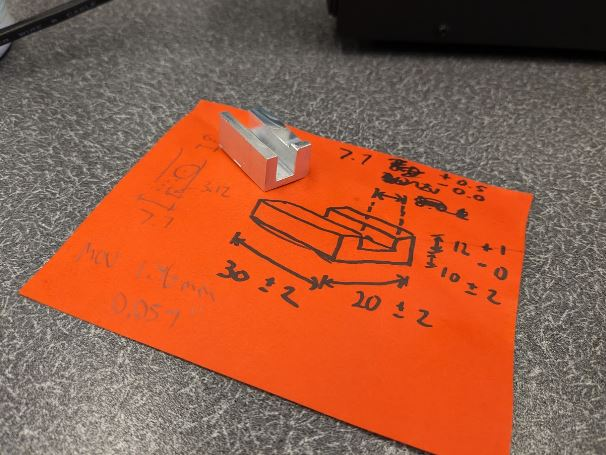
\includegraphics[width=0.9\textwidth]{gaugedrawing}
	\caption{Go/no-go gauge drawing and part}
	\label{fig:gaugedrawing}
\end{figure}

\begin{figure}[htbp]
	\centering
	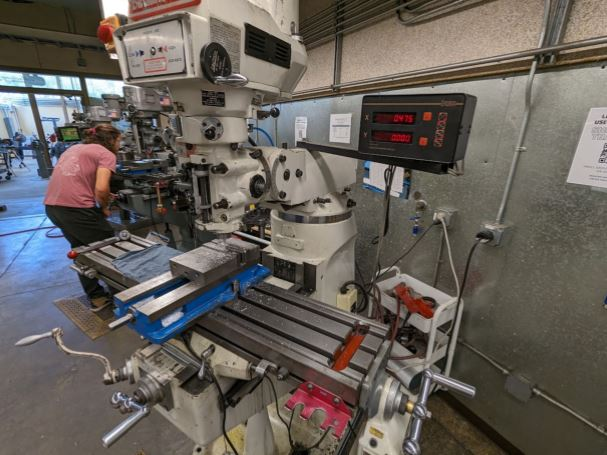
\includegraphics[width=0.9\textwidth]{mill}
	\caption{Manufacturing of go/no-go gauge on mill in Mustang ‘60 Machine Shop}
	\label{fig:mill}
\end{figure}

\noindent Each pair of servos was leveled according to the following workflow:

\begin{itemize}[noitemsep,topsep=0pt]
	\item Set all platforms to a setpoint (0, 0, 10, 0, 0, 0) where all servos should be level, power the Fo-SHIP, and move the platforms to the setpoint
	\item Test each pair of servos with the gauge by attempting to fit the width of both servo horn arms between the channel of the gauge
	\item If little-to-no force is required to fit the servo horn arms between the gauge’s channel, then that pair of servos is level
	\item If a moderate amount of force is required to fit the arms or if they are unable to fit in the gauge, then the servo offsets in \verb|const int PW_OFFSET[]| in \verb|Hexapod_Config1.h| need to be adjusted.
	\item Adjust the servo offsets by a small amount in the direction of the misalignment; if both servo arms have a downward slope from the base to the tip of the servo horn, then add an offset that will make the servos turn upright
	\item Repeat this process, applying the new offset values and testing each pair of servos, until all servo horns are level
\end{itemize}

Each servo horn is between 7.5mm and 7.8mm in width and between 24.5mm and 25.5mm in length between connection holes. The go-no-go gauge has a width of 7.85mm and a length of 31.4mm. The spacing between servos is between 57mm and 59mm. In a worst-case scenario, both servo horns are 7.5mm wide and 24.5mm long, and the spacing between servos is 59mm. The relationship between these constants and the maximum angular misalignment between the servos is derived below.

\begin{figure}[htbp]
	\centering
	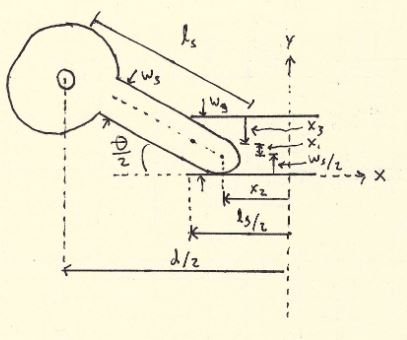
\includegraphics[width=0.9\textwidth]{misalign}
	\caption{Servo misalignment diagram (exaggerated scale)}
	\label{fig:misalign}
\end{figure}

The goal is to find an equation that relates the angle $\theta$ to the constants of the physical setup. By comparing the vertical components of the servo horn arm with the width of the gauge, we can find the following equations:

\begin{equation}\label{eq:2eq14}
	x_2 = \frac{d}{2} - l_s cos(\frac{\theta}{2})
\end{equation}

\begin{equation}\label{eq:2ew15}
	x_1 = (\frac{l_g}{2} - x_2) * \frac{sin(\frac{\theta}{2})}{cos(\frac{\theta}{2})}
\end{equation}

\begin{equation}\label{eq:2eq16}
	x_3 = \frac{w_s}{2cos(\frac{\theta}{2})}
\end{equation}

\begin{equation}\label{eq:2eq17}
	w_g = \frac{w_s}{2} + x_1 + x_3
\end{equation}

This system of equations was solved using the worst-case scenario constants from above using Python to get a maximum angular error of 3.7° between servos when using the go/no-go gauge. This angular misalignment is a worst-case and not all servos are misaligned to this degree, but it’s important to take into consideration when performing the position estimate validation.

\begin{lstlisting}[language=C++]
import numpy as np
from scipy.optimize import fsolve

# Givens
ws = 7.5
ls = 24.5
wg = 7.85
lg = 31.4
d = 59

# Calculate
def equations(vars):
theta = vars
x2 = d/2 - ls * np.cos(theta/2)
x1 = (lg/2 - x2) * np.sin(theta/2) / np.cos(theta/2)
x3 = ws / (2 * np.cos(theta/2))
eq1 = ws/2 + x1 + x3 - wg
return eq1

theta_ans = fsolve(equations, (0))  # Initial guess
print(np.degrees(theta_ans))
\end{lstlisting}

\section{System Testing and Validation} \label{sec:2s7}
Once the servos were calibrated and all of the code was functioning, it was imperative to verify the accuracy of the Fo-SHIP’s position estimate. A variety of positions were tested and measured multiple times, and the averages of these measurements were recorded. Table \ref{tab:foshipvalid} summarizes the positions tested, the estimated XYZ position of the iSBL array’s center, and the measured XYZ position of the iSBL array’s center. The measured values have an uncertainty of ±1.6mm due to the measurement devices used. All units are in millimeters, and the absolute error is computed as the L2 distance from the estimated point to the measured point. The estimated XYZ position is calculated using the forward kinematics model described in Section \ref{ssec:2s5s4} and uses the IMU on the iSBL array for orientation estimation.

\begin{table}[htbp]
	\centering
	\caption{Fo-SHIP position validation}
	\label{tab:foshipvalid}
	\renewcommand{\arraystretch}{1.2}
	\begin{tabular}{|c|c|c|c|c|c|c|c|}
		\hline
		Position & Est. X & Est. Y & Est. Z & Meas. X & Meas. Y & Meas. Z & Abs. Err. \\
		\hline
		Zero & 124 & 1 & -642 & 127 & 0 & -643 & 3.32 \\
		\hline
		Max X & 152 & 1 & -638 & 152 & 2 & -639 & 1.41 \\
		\hline
		Max Y & 126 & 21 & -642 & 127 & 19 & -643 & 2.45 \\
		\hline
		Min Z & 122 & -2 & -708 & 126 & -1 & -711 & 5.10 \\
		\hline
		Max Roll & 90 & 305 & -520 & 101 & 295 & -535 & 21.12 \\
		\hline
		Min Pitch & 333 & 4 & -425 & 340 & 2 & -430 & 8.83 \\
		\hline
		Med Roll & 111 & 178 & -604 & 105 & 172 & -610 & 10.39 \\
		\hline
		Med Pitch & 263 & 2 & -542 & 257 & 1 & -543 & 6.16 \\
		\hline
	\end{tabular}
\end{table}

The average positional error of the Fo-SHIP when using the IMU orientation compensation is 7.35mm. The maximum error measured was 21.12mm (for the maximum possible displacement), and the positional error tends to grow as the pitch and roll increase.

\noindent This error comes from a variety of sources:

\begin{itemize}[noitemsep,topsep=0pt]
	\item Angular misalignment for the servo horns, as described in the previous section
	\item Slop in the system from servos not holding their precise angle due to loading
	\item Potentially loose connections from the heat-set inserts moving during testing
	\item Slight bending on some of the threaded rod linkages from repeated testing
	\item Inaccurate measurement of parameters for a single platform as defined in the code
	\item Measurement inaccuracy from above testing
\end{itemize}

While this error is larger than desired, it is acceptable given the low-cost nature of the actuator. Better actuators and metal base plates would significantly improve the positioning accuracy of the Fo-SHIP. For any future implementations, it is recommended to use linear actuators in place of rotational servos and to use machined metal plates with smaller tolerances than the 3D printed components used here.

\bibliographystyle{IEEEtran}
\bibliography{../thesis}

\end{document}